\chapter{Singlets from the diffuse search}

Two singlets were found to pass in the \gls{vpol} channel of the diffuse search as described in Chapter~\ref{results_diffuse}. These singlets belonged to bins 2998 and 3037, respectively. Information on the events is shown again in Table~\ref{vpol_singlets}. Note that in the bins 2998 and 3037, I had to remove one and three blasts, respectively, by hand after the LD cut. 

Magic display waveforms for the singlet events are shown below. 
Waveforms recorded by each antenna for singlet event 21702154 are shown in Figure~\ref{21702154_wave}. Waveforms recorded in the \gls{vpol} channel are shown at the top and waveforms in the \gls{hpol} channel are shown at the bottom. It can be seen that this event passed the trigger in both \gls{vpol} and \gls{hpol}. 

Distributions for these bins are shown in Figures~\ref{2998_10pc},~\ref{3037_10pc},~\ref{2998_90pc}, and~\ref{3037_90pc} using either the 10\% or 90\% sample of events before final cuts. Final cuts include the LD cut, bin cut, and event bin-weight cut. 

\begin{table}
\centering
\begin{tabular}{ |c|c|c|c|c|c|c|c| } 
\hline
Event & Pol & Run & Bin & Bin-Weight & Latitude & Longitude\\
\hline
21702154 & V & 207 & 3037 & 1.0 & -82.7 & 118.4\\
73750661 & V & 397 & 2998 & 0.9 & -77.3 & 163.4\\
\hline
\end{tabular}
\caption{My singlets from the diffuse search.}
\label{vpol_singlets}
\end{table}



\begin{figure}
\centering
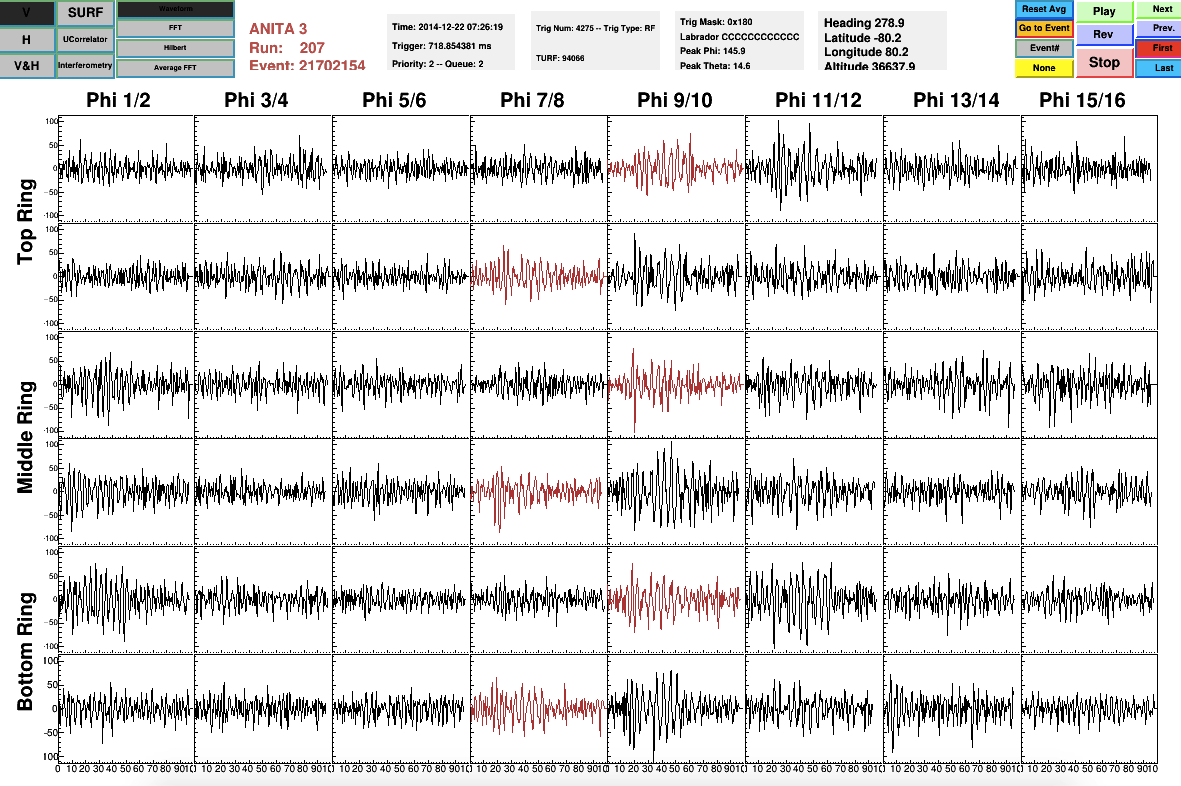
\includegraphics[width=0.9\textwidth]{figures/21702154V.png}
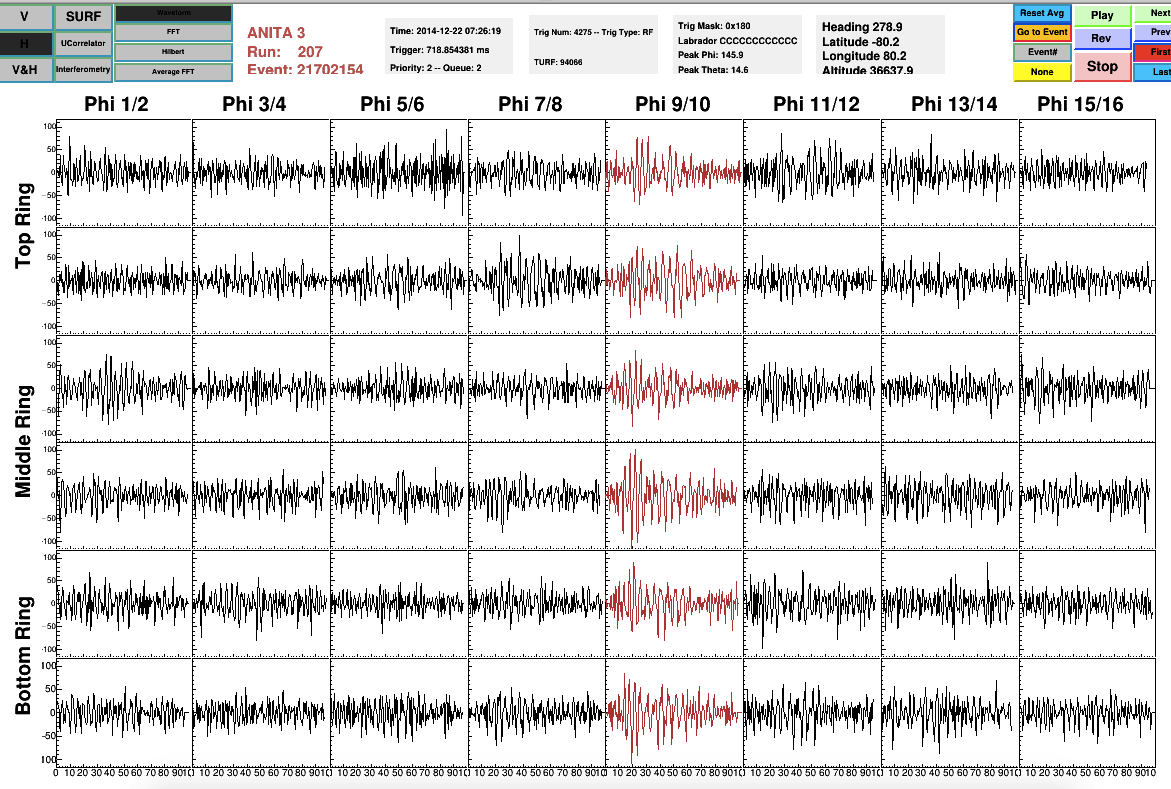
\includegraphics[width=0.9\textwidth]{figures/21702154H.png}
\caption{Waveforms in VPol (top) and HPol (bottom) for singlet event 21702154.}
\label{21702154_wave}
\end{figure}



\begin{figure}
\centering
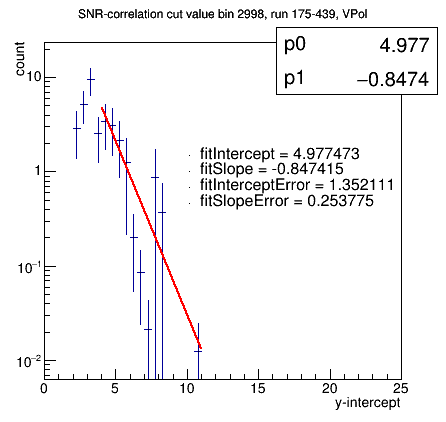
\includegraphics[width=1.0\textwidth]{figures/cutValHistV02998.png}
\caption{Distribution and exponential fit for bin 2998 using the 10\% dataset or burn sample before final cuts. This is the distribution based on which the optimized LD cut for this bin was determined.}
\label{2998_10pc}
\end{figure}


\begin{figure}
\centering
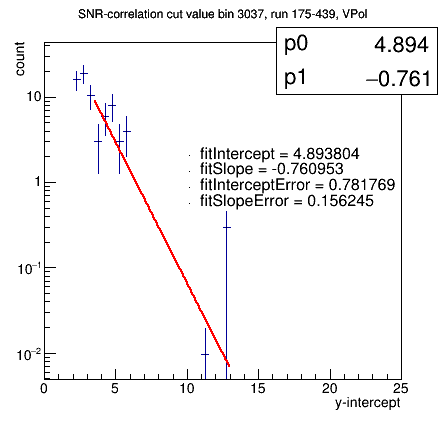
\includegraphics[width=1.0\textwidth]{figures/cutValHistV03037.png}
\caption{Distribution and exponential fit for bin 3037 using the 10\% dataset or burn sample before final cuts. This is the distribution based on which the optimized LD cut for this bin was determined.}
\label{3037_10pc}
\end{figure}


\begin{figure}
\centering
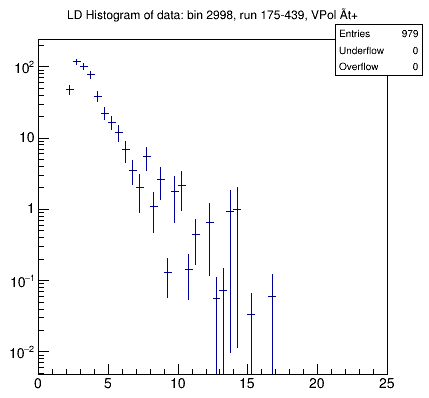
\includegraphics[width=1.0\textwidth]{figures/diffHist02998_175_439_V.png}
\caption{Distribution and exponential fit for bin 2998 using the 90\% dataset before final cuts. Passing singlet event 73750661 belongs to this distribution.}
\label{2998_90pc}
\end{figure}



\begin{figure}
\centering
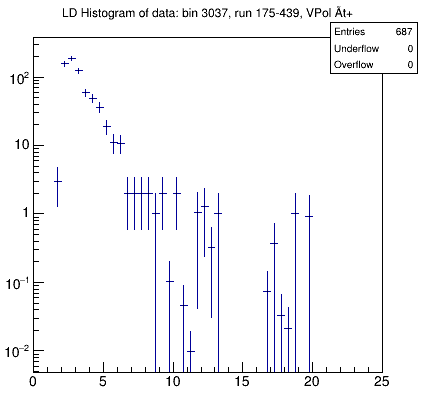
\includegraphics[width=1.0\textwidth]{figures/diffHist03037_175_439_V.png}
\caption{Distribution and exponential fit for bin 3037 using the 90\% dataset before final cuts. Passing singlet event 21702154 belongs to this distribution.}
\label{3037_90pc}
\end{figure}





